\section{Model Results}
	Given a coordinate input of the locations of participants and the time of year, our model optimizes the location for a meeting and predicts the total ticket costs. Since the exact coordinate is not necessarily a city, the nearest city with an airport city was selected as the best location. 

The top coordinates for each scenario are shown, and if a nearby airport exists, it is shown as well.\\


Scenario 1\\
52.1863724, 93.1053239 - Kyzyl Airport, Kyzyl, Russia\\
52.1863724, 88.1053239\\
52.1863724, 98.1053239\\
47.1863724, 88.1053239 - Altay Airport, Altay, Xinjiang, China\\
52.1863724, 103.105324 - International Airport Irkutsk, Irkutsk, Russia\\
47.1863724, 93.1053239\\
52.1863724, 83.1053239\\
47.1863724, 83.1053239 - Tacheng Airport, Tacheng Prefecture, China\\
52.1863724, 108.105324 - Baikal International Airport, Ulan-Ude, Russia\\

Scenario 2\\
52.1863724, 73.9411199 - Astana International Airport, Astana, Kazakhstan\\
52.1863724, 68.9411199 - Kokshetau Airport, Kokshetau, Kazakhstan\\
52.1863724, 78.9411199\\
52.1863724, 63.9411199 - Kostanay Airport, Kostanay, Kazakhstan\\
47.1863724, 73.9411199 - Balkhash Airport, Balkhash, Kazakhstan\\
47.1863724, 78.9411199 - \\
47.1863724, 68.9411199 - Zhezhazgan Airport, Zhezqazgan, Kazakhstan\\

	Typically, the predicted latitudinal coordinate $\approx$ average latitudinal location of the participants. However, the optimal longitudinal location tended towards the western side so that there would be more western travel than eastern travel. In our model, this is due to the dependence of the severity of jet lag begin on direction. Similarly to a study conducted by Lu et al, our model showed that eastward travel caused more loss of productivity from jet lag than westward travel. We conducted a paired t-test to compare the severity of jet lag from eastward travel and westward travel. The severity of jet lag from eastward jet lag was significantly greater than the severity of westward jet lag (\textit{p} = 0.002, df = 58, \textit{t} = 2.00). Locations that required less eastward travel were more optimal. 
	Below is a map of our results and the input for both scenarios. 
\begin{figure}
\includegraphics[width=\textwidth]{scenario1.eps}
\caption{Scenario 1}
\end{figure}

\begin{figure}
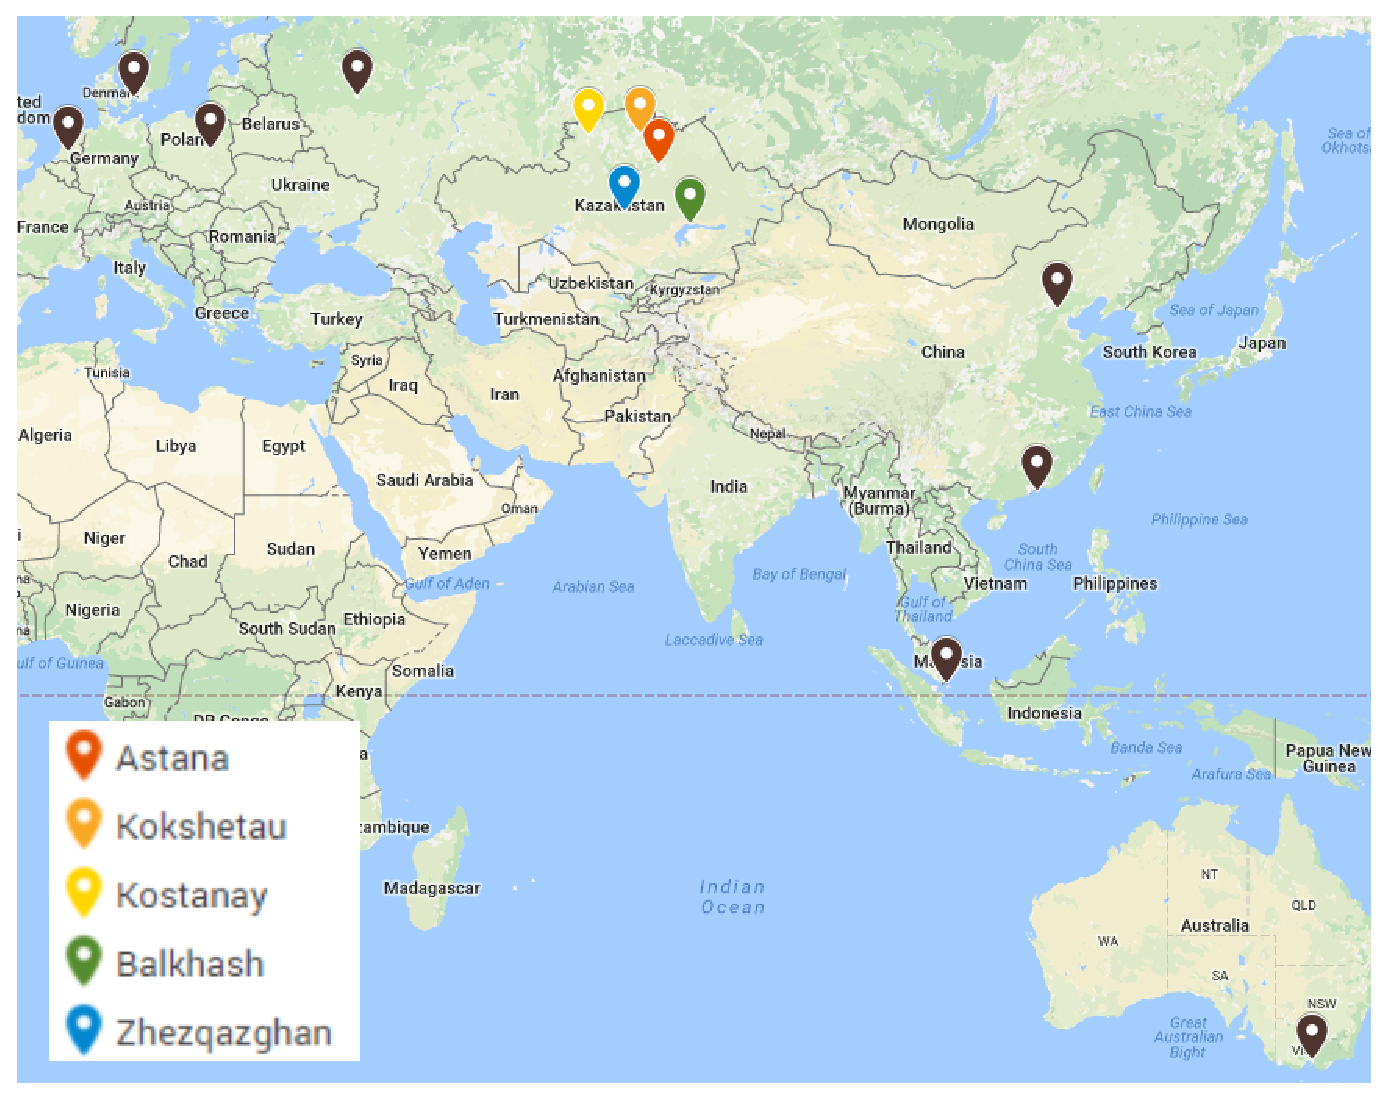
\includegraphics[width=\textwidth]{scenario2.eps}
\caption{Scenario 2}
\end{figure}

\begin{figure}[h!]
\includegraphics[width=\textwidth]{LAXtoNRTprice.eps}
\caption{gradient descent regression}
\end{figure}

\begin{figure}[h!]
	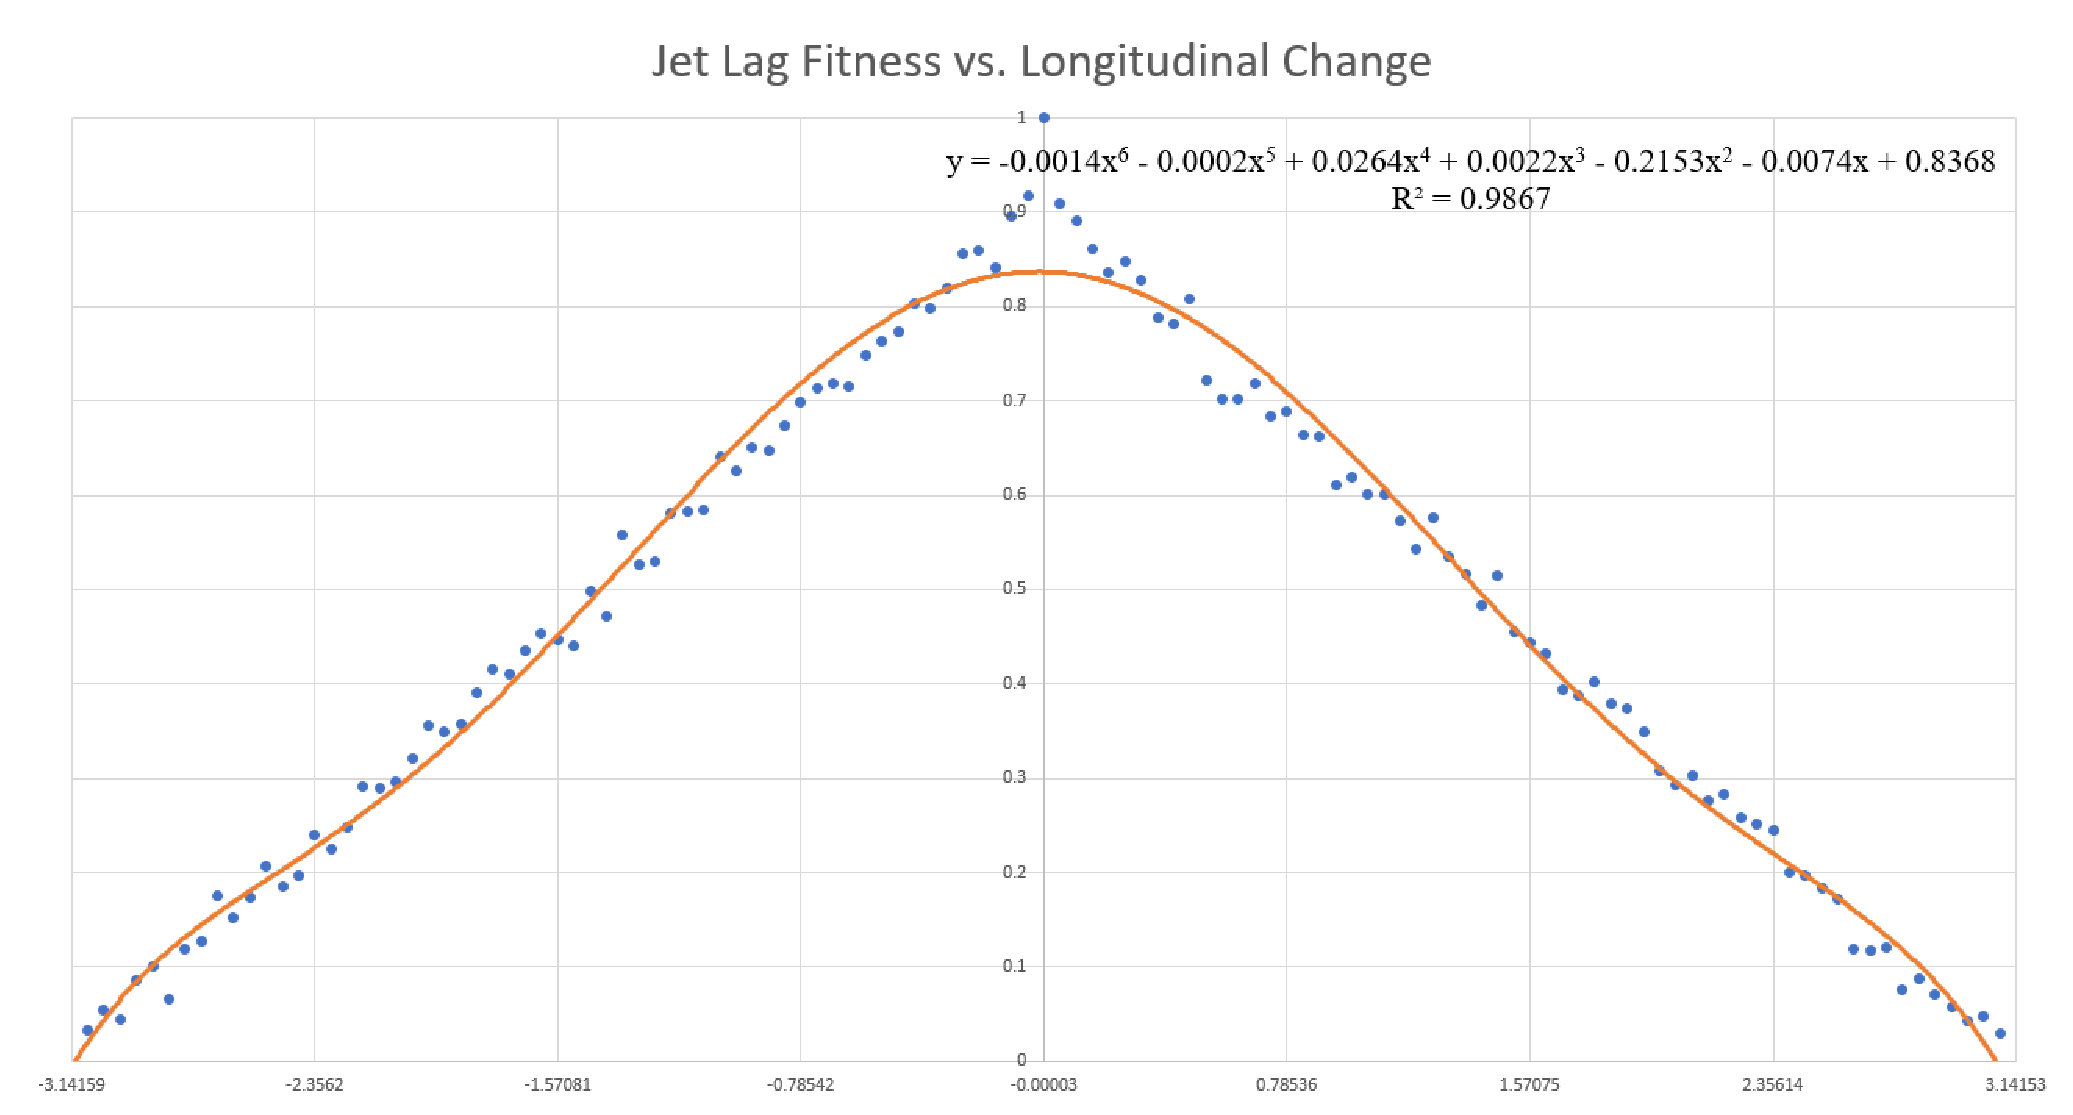
\includegraphics[width=\textwidth]{kuramotofitnessgraph.eps}
	\caption{$t$ required for no jet lag for different values of $\Delta(p)$}
\end{figure}	
